\documentclass[xcolor=table, unknownkeysallowed]{beamer}

\newcommand\Fontvi{\fontsize{9}{10.2}\selectfont}

\mode<presentation> {

\usetheme{Madrid}
\setbeamertemplate{navigation symbols}{}
}

\usepackage{graphicx} % Allows including images
\usepackage{booktabs} % Allows the use of \toprule, \midrule and \bottomrule in tables

\usepackage{subfigure}
\usepackage{textpos}
\usepackage{pifont} 
\usepackage{algorithm}
\usepackage[noend]{algpseudocode}
\usepackage[T1]{fontenc}
\usepackage{fancyref}
\usepackage{float}
\usepackage{times}
\usepackage{epsfig}
\usepackage{graphicx}
\usepackage{amsmath}
\usepackage{amssymb}
\usepackage{url}
\usepackage{xcolor}
\usepackage{media9}
\usepackage{multimedia}
\setbeamertemplate{itemize item}{\scriptsize\ding{108}}
\setbeamertemplate{itemize subitem}{\scriptsize\ding{117}}

\addtobeamertemplate{frametitle}{}{%
\begin{textblock*}{10cm}(.85\textwidth,-1cm)
\hspace{-3.25cm}
\includegraphics[height=1cm]{img/logo_blu.jpeg}
\end{textblock*}}


\title[Twitter real-time sentiment analysis]{Lambda Architecture for Twitter real-time sentiment analysis} % The short title appears at the bottom of every slide, the full title is only on the title page

\author{Lorenzo Agnolucci} % Your name
\institute[] % Your institution as it will appear on the bottom of every slide, may be shorthand to save space
{
Universit\`a degli Studi di Firenze \\ % Your institution for the title page
Dipartimento di Ingegneria dell'Informazione \\
 % Your email address
}
\date{Firenze, 20 Aprile 2019} % Date, can be changed to a custom date

\begin{document}


\begin{frame}
\titlepage % Print the title page as the first slide
\begin{figure}
    \centering
    \includegraphics[width=0.2\textwidth]{img/stemma.pdf}
\end{figure}
\end{frame}

%----------------------------------------------------------------
%----------------------------------------------------------------

\begin{frame}
\frametitle{Outline}
\tableofcontents
\end{frame}

%----------------------------------------------------------------
%----------------------------------------------------------------

\section{Introduction}

\begin{frame}
\frametitle{Introduction}
\begin{itemize}
\item Big Data requires to find ways to analyze a large amount of data
\vspace{0.25cm}
\item Lambda Architecture is a particular approach composed by:
\vspace{0.15cm}

\begin{itemize}
\item \emph{batch layer} : applies batch-oriented technologies (like MapReduce) on a master database. It is effective but it has a high latency
\vspace{0.15cm}
\item \emph{serving layer} : specialized distributed database that supports batch updates and random reads
\vspace{0.15cm}
\item \emph{speed layer} : only looks at recent data and uses low-latency techniques to update real-time views. It compensate for the high latency of the batch layer
\end{itemize}
\vspace{0.25cm}

\item Sentiment analysis is a type of data mining applied to Big Data with some useful applications
\end{itemize}
\end{frame}

%----------------------------------------------------------------
%----------------------------------------------------------------

\section{Proposed approach}

\begin{frame}
\frametitle{Proposed approach}
\begin{figure}
\centering
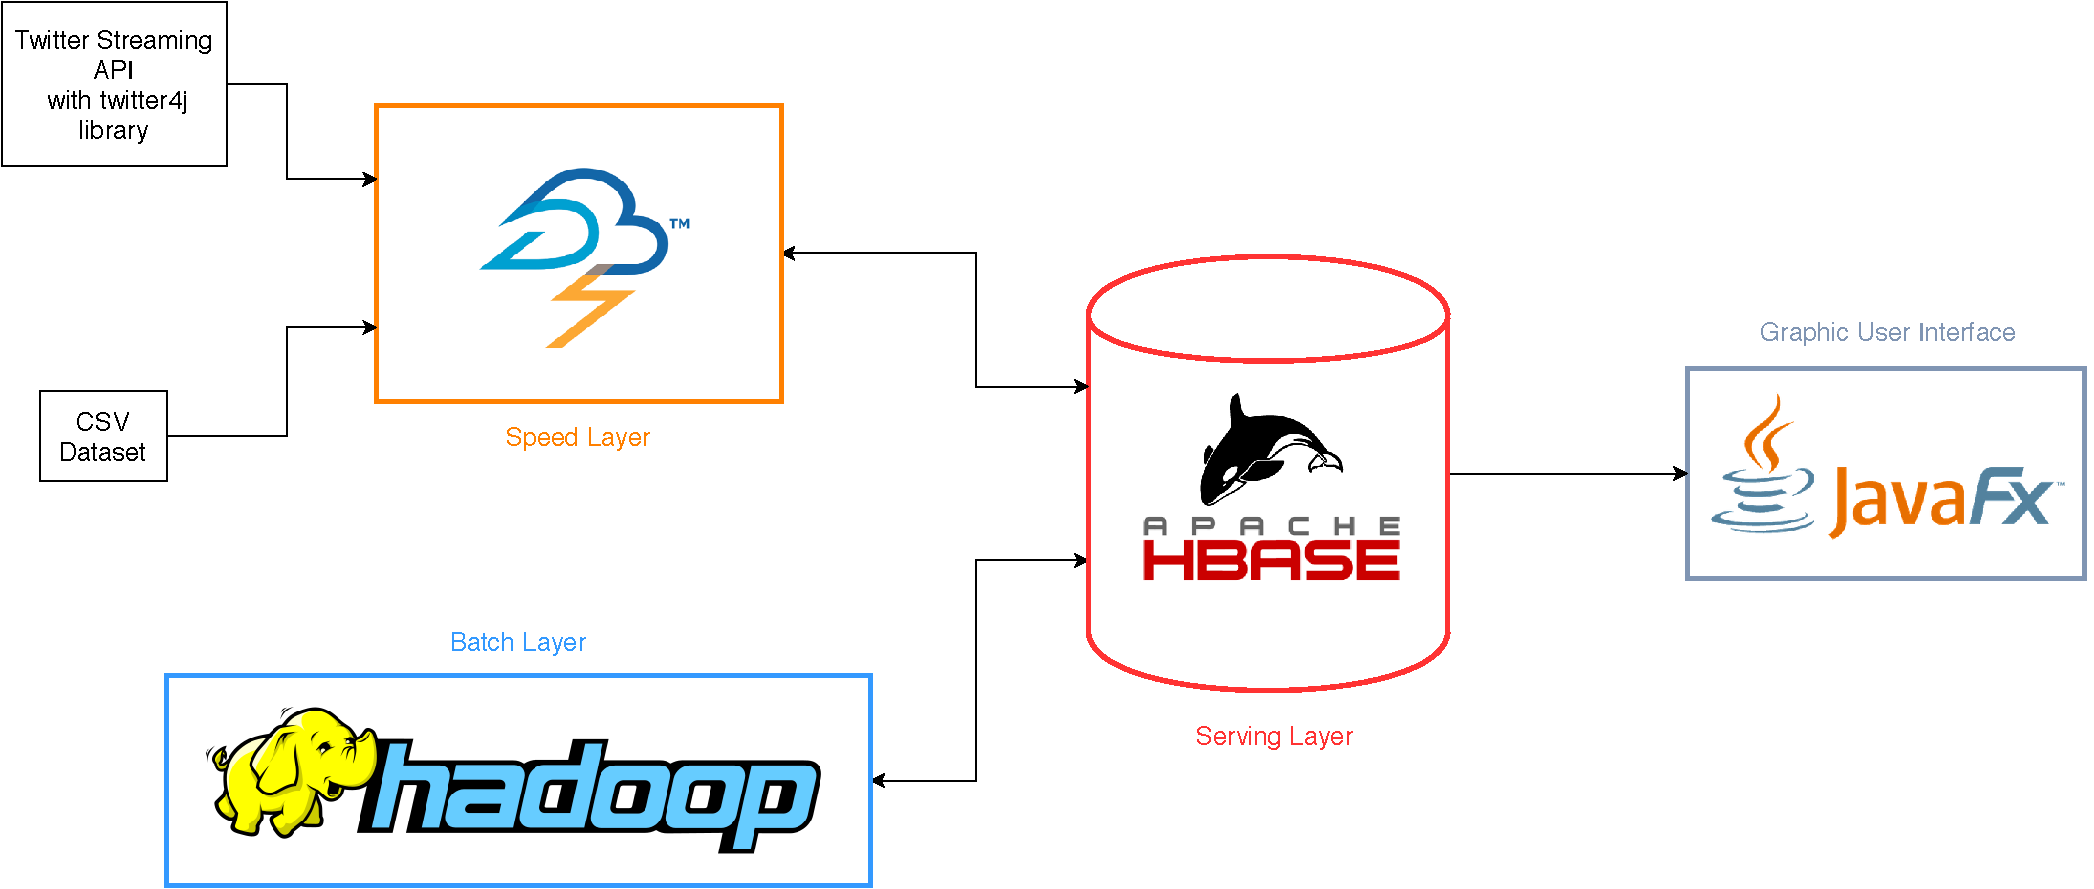
\includegraphics[width=0.85\linewidth]{img/lambda_architecture_diagram}
\label{fig:lambda_architecture_diagram}
\end{figure}
\begin{itemize}
\item The main goal was not a perfect sentiment classification but the implementation of the architecture
\item Speed layer is started first with the keywords as arguments. It creates the speed layer tables at the start of the execution
\item Tweets of a dataset are added as if they belonged to the real-time stream to increase the number of tweets
\end{itemize}
\end{frame}

%----------------------------------------------------------------
%----------------------------------------------------------------

\subsection{Sentiment classifier}

\begin{frame}
\frametitle{Sentiment classifier}
\begin{itemize}
\item Developed with \emph{LingPipe} library
\vspace{0.5cm}
\item Trained on 1.6 millions tweets \footnote{\tiny{A. Go, R. Bhayani, and L. Huang. Twitter sentiment classification using distant supervision. CS224N project report, Stanford, 1(12):2009, 2009. https://www.kaggle.com/kazanova/sentiment140}}
\vspace{0.5cm}
\item Classifies English text with 2 categories: positive and negative
\vspace{0.5cm}
\item Decent 0.71 accuracy
\end{itemize}
\end{frame}

%----------------------------------------------------------------
%----------------------------------------------------------------

\subsection{Serving layer}

\begin{frame}
\frametitle{Serving layer}

Based on Apache HBase and composed by 4 tables:
\vspace{0.5cm}
\begin{itemize}
\item \emph{tweet master database}: master database of the Lambda Architecture
\vspace{0.25cm}
\item \emph{tweet real-time database}: stores the tweets on which the real-time view is based
\vspace{0.25cm}
\item \emph{batch view}: result of the batch processing
\vspace{0.25cm}
\item \emph{synchronization table}: contains the start and the end timestamps of the batch processing
\end{itemize}
\end{frame}

%----------------------------------------------------------------
%----------------------------------------------------------------

\subsection{Batch layer}

\begin{frame}
\frametitle{Batch layer}

\begin{itemize}
\item Represented by Apache Hadoop
\vspace{0.15cm}
\item Computes a MapReduce job on \emph{tweet master database} in a infinite loop
\vspace{0.15cm}
\item Writes its results from scratch in \emph{batch view}
\vspace{0.15cm}
\item Writes the start and the end timestamps of the computation in \emph{synchronization table}
\vspace{0.15cm}
\item Mapper takes a tweet in input and outputs a $<Keyword, Sentiment>$ tuple
\vspace{0.15cm}
\item Reducer takes a tuple in input and increment the corresponding cell in \emph{batch view}
\end{itemize}
\end{frame}

%----------------------------------------------------------------
%----------------------------------------------------------------

\subsection{Speed layer}

\begin{frame}
\frametitle{Speed layer}
\vspace{-0.45cm}
\begin{figure}
\includegraphics[width=0.95\linewidth]{img/storm_topology_diagram}
\label{fig:storm_topology_diagram}
\end{figure}
\begin{itemize}
\item \emph{tweet stream spout}: gets a real-time stream of tweets with \emph{Twitter4j} library and filters them
\vspace{0.15cm}
\item \emph{tweet parser bolt}: parse a tweet object to a tuple
\end{itemize}
\end{frame}

%----------------------------------------------------------------
%----------------------------------------------------------------

\begin{frame}
\frametitle{Speed layer}
\vspace{-0.5cm}
\begin{figure}
\includegraphics[width=0.95\linewidth]{img/storm_topology_diagram}
\label{fig:storm_topology_diagram}
\end{figure}
\begin{itemize}
\item \emph{tweet CSV spout}: outputs a tuple for each tweet of the dataset
\vspace{0.15cm} 
\item \emph{master database mapper bolt}: inserts tweets in \emph{tweet master database}
\end{itemize}
\end{frame}

%----------------------------------------------------------------
%----------------------------------------------------------------

\begin{frame}
\frametitle{Speed layer}
\vspace{-0.275cm}
\begin{figure}
\includegraphics[width=0.95\linewidth]{img/storm_topology_diagram}
\label{fig:storm_topology_diagram}
\end{figure}
\begin{itemize}
\item \emph{tweet sentiment classifier bolt}: classifies the sentiment of the tweet
\vspace{0.15cm}
\item \emph{real-time database mapper bolt}: inserts tuples in \emph{tweet real-time database}
\end{itemize}
\end{frame}

%----------------------------------------------------------------
%----------------------------------------------------------------

\begin{frame}
\frametitle{Speed layer}
\vspace{-0.5cm}
\begin{figure}
\includegraphics[width=0.95\linewidth]{img/storm_topology_diagram}
\label{fig:storm_topology_diagram}
\end{figure}
\begin{itemize}
\item \emph{synchronization spout}: checks when batch processing ends
\vspace{0.15cm}
\item \emph{synchronization bolt}: deletes already processed tweets from \emph{tweet real-time database}
\end{itemize}
\end{frame}

%----------------------------------------------------------------
%----------------------------------------------------------------

\subsection{GUI}

\begin{frame}
\frametitle{GUI}
\begin{center}
    \movie[showcontrols, loop]{\includegraphics[width=0.86\textwidth]{img/GUI}}{img/GUI_video.mp4}
  \end{center}
\end{frame}

%----------------------------------------------------------------
%----------------------------------------------------------------

\section{Conclusions}

\begin{frame}
\frametitle{Conclusions}
\begin{itemize}
\item It has been shown an implementation of a Lambda Architecture capable of getting sentiment analysis statistics of real-time tweets
\vspace{0.75cm}
\item The GUI that was developed lets to visualize how the different parts of the architecture work together
\vspace{0.75cm}
\item As a future development a neutral category could be added to the sentiment classifier
\end{itemize}
\end{frame}

\end{document} 